\section{Dataset and Preprocessing}

The quality of a prediction model heavily depends on the quality and processing of input data. This section describes the data source, exploratory analysis, collected features, and preprocessing steps performed.

\subsection{Data Source}

The data used in this project is the "Survey Lung Cancer" dataset that collects information about risk factors and symptoms related to lung cancer. The initial dataset included 309 samples and 16 features. After removing duplicate records, 276 unique samples remained for analysis and model training.

\subsection{Exploratory Data Analysis (EDA)}

Several exploratory analyses were conducted to better understand the data characteristics, particularly in the group of patients diagnosed with lung cancer.

\begin{figure}[H] % Using [H] to try to keep the image in place
    \centering
    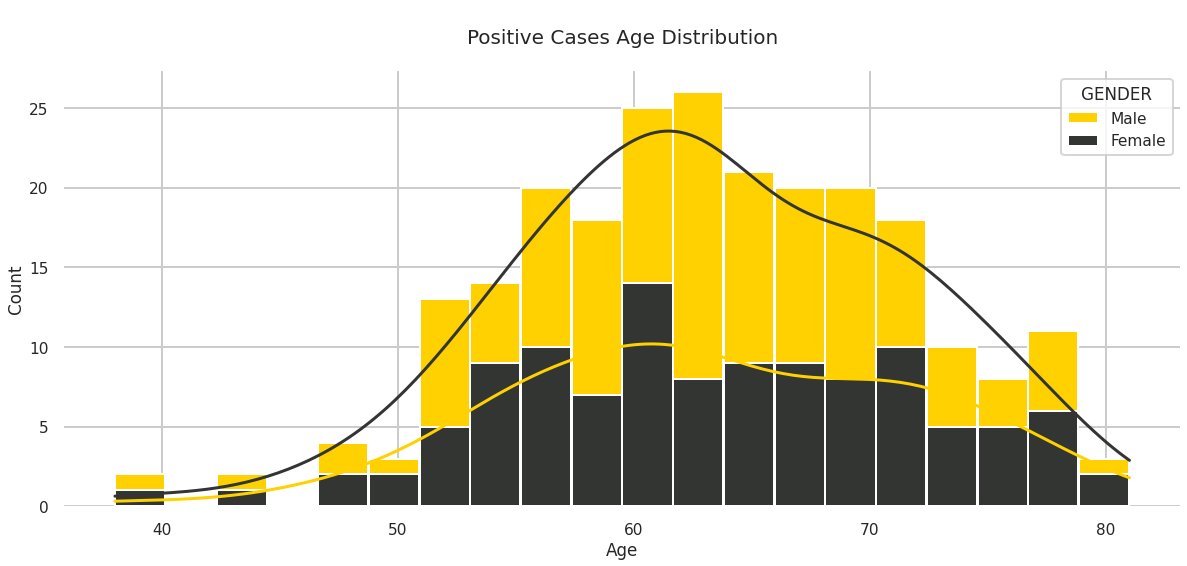
\includegraphics[width=0.8\textwidth]{Images/positive_cases_age_dist.png}
    \caption{Age distribution of positive cases, separated by gender.}
    \label{fig:age_dist}
\end{figure}

As shown in Figure \ref{fig:age_dist}, the age distribution of lung cancer cases shows a clear peak in the 60-70 age range for both males and females. This distribution follows a curve similar to normal distribution, with low frequency in age groups below 50 and above 80. Notably, the proportion of males (yellow color) is higher in most age groups, especially in the 55-65 age range. Overall, this distribution confirms that lung cancer is more common in older people and tends to affect males more, which is consistent with epidemiological studies of lung cancer.

\begin{figure}[H]
    \centering
    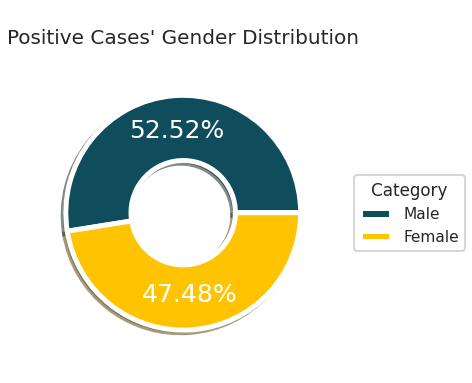
\includegraphics[width=0.5\textwidth]{Images/gender.png}
    \caption{Gender distribution in positive cases.}
    \label{fig:gender_dist}
\end{figure}

Figure \ref{fig:gender_dist} shows the gender ratio in lung cancer positive cases. The pie chart indicates that males account for 54.55\% and females for 45.45\% of total cases. The higher proportion of males in this dataset reflects the general trend in lung cancer studies, possibly due to risk factors related to males (such as higher smoking rates) or genetic and physiological factors.

\begin{figure}[H]
    \centering
    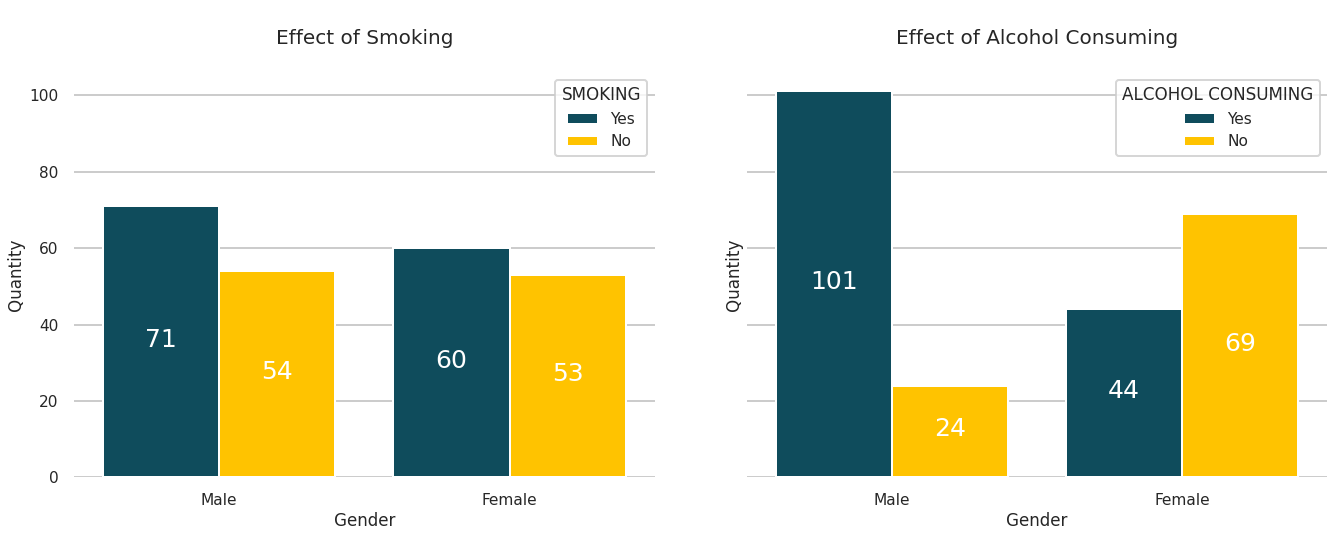
\includegraphics[width=\textwidth]{Images/smoke_alcohol.png}
    \caption{Comparison of smoking and alcohol consumption rates in positive cases by gender.}
    \label{fig:smoke_alcohol}
\end{figure}

Figure \ref{fig:smoke_alcohol} provides insight into two main risk factors for lung cancer: smoking and alcohol use, broken down by gender. The left chart shows a large number of male lung cancer patients who smoke (51 cases), compared to non-smokers (20 cases). For females, the ratio is similar but with lower numbers (38 smoking cases and 18 non-smoking cases).

Similarly, the right chart shows alcohol usage patterns, with a similar but less pronounced pattern than smoking. In both genders, alcohol users make up the majority of lung cancer cases, with 43 males and 32 females who use alcohol compared to 28 males and 24 females who don't. These results highlight the recognized connection between lifestyle habits such as smoking and drinking and lung cancer risk.

\begin{figure}[H]
    \centering
    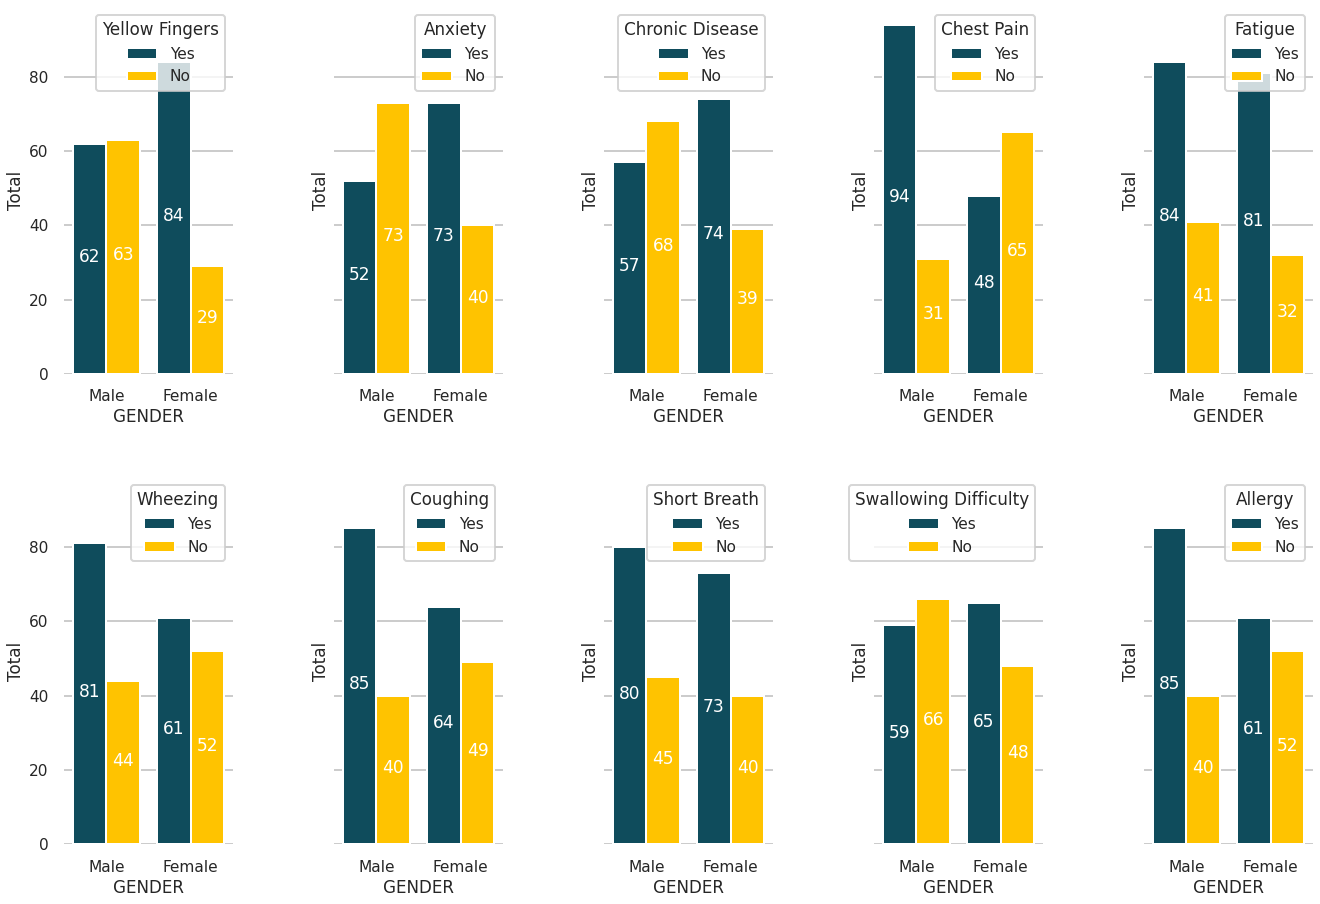
\includegraphics[width=\textwidth]{Images/symptoms.png}
    \caption{Distribution of symptoms and risk factors in positive cases by gender.}
    \label{fig:symptoms_dist}
\end{figure}

Figure \ref{fig:symptoms_dist} provides a detailed overview of the prevalence of different symptoms in lung cancer patients, broken down by gender. From this chart, several key points can be observed:

\begin{itemize}
    \item \textbf{Anxiety:} A common symptom in both males and females, with a high positive rate (especially in males).
    \item \textbf{Yellow Fingers:} This sign appears in about 2/3 of patients, reflecting the effects of long-term cigarette smoking.
    \item \textbf{Fatigue:} A very common symptom in both genders, especially in females, indicating this is an important symptom to monitor.
    \item \textbf{Shortness of Breath and Coughing:} These two classic respiratory symptoms are present in over 50\% of patients, but not all, highlighting the challenge in diagnosis based solely on clinical symptoms.
    \item \textbf{Chest Pain:} Another concerning symptom appearing in about half of patients.
\end{itemize}

It's noteworthy that most symptoms appear in both genders, but the rates may differ. This suggests that although the basic symptoms are similar, the clinical presentation of lung cancer may have differences between males and females, requiring a personalized approach to diagnosis and treatment.

Correlation analysis (Figure \ref{fig:correlation_matrix} - see Appendix if available) shows some notable correlations between symptoms, such as between Allergy and Wheezing, or between Coughing and Shortness of Breath.

\subsection{Collected Features and Encoding}

The following features were collected and encoded:
\begin{itemize}
    \item \textbf{Demographics:} Gender (GENDER - Encoded: 'M' to 'Male', 'F' to 'Female', then one-hot encoded into `MALE` and `FEMALE`), Age (AGE - kept as numeric).
    \item \textbf{Lifestyle and Symptoms:} The remaining variables (SMOKING, YELLOW\_FINGERS, ANXIETY, etc.) originally had values of 2 (Yes) and 1 (No). They were kept in this numeric form during XGBoost model training because tree-based algorithms can handle these types of categorical variables.
    \item \textbf{Target Label:} Lung cancer diagnosis (LUNG\_CANCER - Encoded: 'YES' to 1, 'NO' to 0).
\end{itemize}

\subsection{Data Preprocessing Steps}

To prepare data for model training, the following steps were performed based on the EDA notebook:
\begin{itemize}
    \item \textbf{Handling Missing Values:} No missing values were detected in this dataset.
    \item \textbf{Removing Duplicates:} 33 duplicate records were removed.
    \item \textbf{Categorical Variable Encoding:} The `GENDER` variable was one-hot encoded. The target variable `LUNG_CANCER` was label encoded.
    \item \textbf{Continuous Variable Standardization:} All input features (including symptom variables with values 1/2 and age) were standardized using `StandardScaler` to have a mean of 0 and standard deviation of 1.
    \item \textbf{Feature Selection and Ordering:} Columns were renamed (e.g., `FATIGUE ` to `FATIGUE`) and reordered in a specific sequence before standardization and training.
\end{itemize}

% \subsection{Feature Engineering}
% No complex feature engineering techniques were applied beyond encoding and standardizing existing variables.

\subsection{Train-Test Data Split}

The dataset was divided into two parts: training set (80\%) and test set (20\%) using `train_test_split` from scikit-learn with `random_state=42`. Although not explicitly mentioned in the notebook about using stratified splitting, this is a good practice for classification problems, especially if there is class imbalance.
